\documentclass[runningheads,a4paper]{llncs}

\usepackage{amssymb}
\setcounter{tocdepth}{3}
\usepackage{graphicx}
\usepackage{booktabs}

\usepackage{url}
% \urldef{\mailcf}\path|{berlin,borazio}@ess.informatik.tu-darmstadt.de, tobias.grosse-puppendahl@igd.fraunhofer.de|
% \newcommand{\keywords}[1]{\par\addvspace\+baselineskip
% \noindent\keywordname\enspace\ignorespaces#1}

\begin{document}

\mainmatter  % start of an individual contribution

% first the title is needed
\title{Enhancing Accelerometer-based Activity Recognition with Capacitive Proximity Sensing}

% a short form should be given in case it is too long for the running head
\titlerunning{Enhancing Accelerometer-based Activity Recognition}
% (feature abused for this document to repeat the title also on left hand pages)
\authorrunning{Enhancing Accelerometer-based Activity Recognition}

% the name(s) of the author(s) follow(s) next
% \author{Tobias Grosse-Puppendahl\inst{1} \and Eugen Berlin\inst{2} \and Marko Borazio\inst{2} }
\author{Author 1 \and Author 2 \and Author 3 }

% the affiliations are given next; don't give your e-mail address
% unless you accept that it will be published
% \institute{
% 	Fraunhofer IGD, Fraunhoferstr. 5, 64283 Darmstadt, Germany\\
% 	\email{tobias.grosse-puppendahl@igd.fraunhofer.de}
% 	\and
% 	Technische Universit\"at Darmstadt, Hochschulstr. 10, 64289 Darmstadt, Germany\\
% 	\email{\{berlin,borazio\}@ess.tu-darmstadt.de}
% }

\institute{
	Anonymized for review \\
	\email{anonymous@insitution.edu}
	\and
	Anonymized for review \\
	\email{anonymous@insitution.edu}
}


% \toctitle{Enhancing Accelerometer-based Activity Recognition with Capacitive Proximity Sensing}
% \tocauthor{Eugen Berlin, Marko Borazio, Tobias Grosse-Puppendahl}

\maketitle
\begin{abstract}
Activity recognition solely with an accelerometer is a common investigated research topic and enables the detection of basic activities like sit, walk or stand. Recent work in this area adds different sensing modalities to the inertial data to collect more information of the users environment and to boost activity recognition.  We present a sensor set-up that consists of an accelerometer and a capacitive proximity sensor that senses the users activity based on the combined sensor values. We show that our proposed approach improves the recognition rate significantly for detecting activities of daily living (e.g. open door, prepare dinner, etc.) by adding capacitive proximity sensor data to the inertial data.
\keywords{ambient assisted living, capacitive proximity sensors, activity recognition, user context}
\end{abstract}

\section{Introduction}

Sensing a persons activity is being researched for several years now, raising even more interest in it by the advanced technology of mobile phones, which include multiple sensors and therefore enable activity recognition with such a device \cite{brezmes2009activity}. Current wearable activity recognition systems are able to unobtrusively capture and recognize a person's activities throughout the whole day. These systems often rely on inertial sensor data that is captured by wearable sensors embedded in a mobile device \cite{brezmes2009activity} or attached to the body \cite{Ravi2005} to identify the activities performed. Usually, single sensor modalities are used or duplicated to detect the activities. However, it is a great challenge to identify fine-grained activities just by using a single modality like the accelerometer. Capacitive proximity sensors on the other hand can indirectly measure the distance and nature of a grounded object within reach. This means that the measurement result depends on the object's distance, its size and the material it is made of. In this work, we show how an accelerometer and a capacitive proximity sensor can be used to improve activity recognition in activities of daily living. For this we obtained a wrist-worn activity data logger\footnote{HedgeHog Activity Logger -- \url{http://www.ess.tu-darmstadt.de/hedgehog}} and integrate a capacitive proximity sensor unobtrusively into the wristband.

There are several intuitive examples for which a combination of accelerometer-based activity recognition with a capacitive proximity sensor reveals its strength. For example, it may be conducted which material is placed underneath the hand. The capacitive proximity sensor would return a different measurement result for a hand placed on a couch covered with fabric than a hand placed a wooden table. Moreover, the approximate distance to objects can be exploited to identify activities like grasping into a locker or a refrigerator to prepare food.

A wristband worn capacitive proximity sensor requires a shield that eliminates the influence of the grounded arm directly underneath the sensor. Using this setup, we can detect the proximity to a grounded object in the environments for distances up to 20 cm. Especially for mobile devices, it is required that the sensor only draws a very small amount of power. Thus, other proximity sensing input modalities like ultrasound or optical measurements are not applicable for this type of mobile application.

This paper is structured as follows: We give a short insight in related work in chapter 2, followed by describing the hardware set-up used for this study in chapter 3. The experiment and evaluation will be described in chapter 4, showing how data has been obtained and how activity recognition is being improved. This work is concluded in chapter 5 with an outlook to future work.

The remainder of this paper is  is structured as follows: First, Section \ref{sect:related} is dedicated to related work work in activity recognition, in particular considering approaches with multiple sensor modalities. Section \ref{sect:hardware} will present the hardware based on which a wrist-worn sensor prototype was built, fusing together an inertial data logger and a capacitive sensor integrated in a wristband. The experimental setup, the scripted scenario with daily activities and the activity recognition evaluation results, showing the performance boost of the capacitive sensor unit, are given in Section \ref{sect:experiment}. The paper is wrapped up with a conclusions section enumerating the findings of the paper, as well as pointing out future research potential.




\section{Related Work}
\label{sect:related}
%%%%%%%%%%%%%%%%%%%%%%%%%%%%%%%%%%%%%%%%%%

Activity recognition research relying on wearable sensors mostly considers inertial data from the participants body to infer performed activities, such as in the works of \cite{Ravi2005,Bao2004,Srinivasan2010,Amft2005}. The acceleration data is often augmented with data from sensors such as gyroscopes \cite{Holleczek_2010}, magnetometers \cite{Altun_2010}, ambient light \cite{Borazio2012} or ambient and skin temperature \cite{Krause_2003}, aiming at extracting more motion and environmental context of the user. Researchers in \cite{wyss2010recognition}, for example, use heart rate information additionally to the accelerometer to detect military related activities like lifting and lowering loads or even digging. In \cite{Ward_2006}, workshop assembly activities were detected by augmenting acceleration sensors with microphones.

The works of \cite{Fishkin_2005} and \cite{patterson2005fga} show that detecting objects the user touches or uses can be very helpful for activity recognition. By using RFID readers that are embedded in gloves or bracelets at the wrist and RFID tags attached to various objects of interest, one can detect the object grasped and used by the user, thus aiding the activity recognition in various application scenarios, such as activities of daily living \cite{phealth:maja} and \cite{Philipose_2004}, activity tracking in car manufacturing \cite{Stiefmeier08}, or household and gardening activities \cite{berlin_laerhoven_tei_2010}. 

Our approach to enhance the inertial data from a wearable sensor is quite similar to the RFID scenarios just mentioned, as it also relies on a single wearable sensor and thus is aiming at an unobtrusive deployment. The main difference lies in the fact that we do not need accurate detection of tagged objects, but are only interested in the proximity to various objects which, as we expect, could boost activity recognition.

% While the RFID gloves or bracelets might not have reached user acceptance, and deploying tags in the user's home might appear cumbersome and still quite intrusive, our approach considers a single wrist-worn sensor unit consisting of an accelerometer and proximity sensor.
% Berlin et al. \cite{berlin_laerhoven_tei_2010} have also fused and benchmarked a wrist-worn accelerometer sensor node with an RFID bracelet to be able to detect objects a human is interacting with, aiming both at household as well as gardening activities.


%%%%%%%%%%%%%%%%%%%%%%%%%%%%%%%%%%%%%%%%%%

\begin{figure}[htbp]
	\centering
		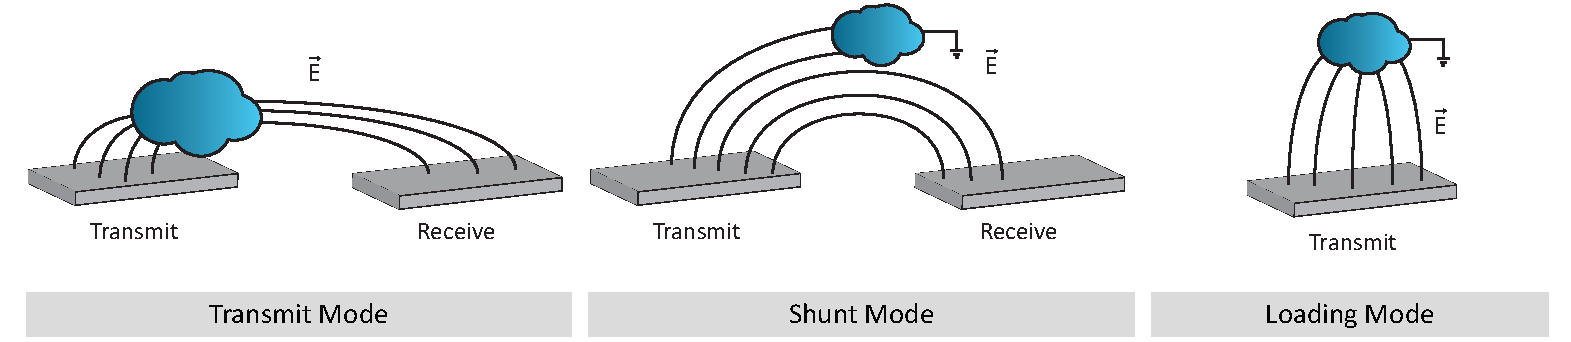
\includegraphics[width=1.00\textwidth]{Images/modes.pdf}
	\caption{Three different capacitive proximity sensing modes can be distinguished \cite{Smith1996}. The sensing electrodes build up an electric field to objects in the environment, illustrated with a cloud.}
	\label{fig:modes}
\end{figure}


In the field of capacitive proximity sensing, three different measurement modes shown in Figure \ref{fig:modes} were identified by Smith et al. \cite{Smith1999}: transmit mode, shunt mode and loading mode. Transmit mode is based on a varying electric potential coupled to an object that can be measured by a capacitive proximity sensor next to that object. Shunt mode applies two electrodes, a transmit and a receive electrode, that can measure capacitance changes produced by objects disturbing the electric field between the two electrodes. In loading mode, a single electrode builds up an electric field to any grounded object in the environment. By measuring the capacitance, conclusions can be made upon the proximity and nature of an object. In our work we apply loading mode since it requires only a single electrode that can be integrated invisibly into the wristband.

A great variety of capacitive sensors and measurement techniques exists \cite{Smith1999}. The most common sensing principle, the loading mode, is based on running numerous charge and discharge cycles of the virtual capacitor that is created by the electrode and the environment. Depending on the charge and discharge times, one can infer the corresponding capacitance. This sensing principle is applied by Wimmer et al. in \cite{Wimmer2007} who presented a toolkit for capacitive proximity sensing.

In previous works, capacitive proximity sensors were applied in various fields of human-computer-interaction. For example, Wimmer et al. and Grosse-Puppendahl et al. presented gesture recognition systems \cite{Wimmer,Grosse-puppendahl2012} as well as smart furniture that can sense human activities \cite{Wimmer} and classify human postures \cite{Grosse-puppendahl2011}. Cheng et al. have investigated the possibility of using capacitive sensors for activity recognition by measuring shape changes of muscles and skin \cite{Cheng2010}. To our knowledge, capacitive proximity sensors have not been embedded into a wearable device to enhance the performance of activity recognition.


\section{Hardware}
\label{sect:hardware}
This section presents the two components of the required hardware, the wrist-worn activity data logger tailored to capture acceleration data, and the capacitive proximity sensor used for distance measurements.

\subsection{Activity Data Logger}
The HedgeHog sensor is a custom designed and built wearable data logger aiming at long-term deployments in activity recognition scenarios. Due to its small form-factor (30x25x20mm) and weight, this sensor, being worn at the wrist, is an unobtrusive way to record relevant motion data.

The sensor node itself is built around the low-power Microchip microcontroller (PIC18F46J50) featuring an accelerometer sensor (ADXL345) to capture human motion, light and ambient temperature sensors and a microSD flash card for locally storing the sensor data. The sensor is powered by a $200mAh$ lithium polymer battery, which allows for two weeks of continuous recording on a single battery charge. A USB port is used to configure the sensor (e.g. setting the sensitivity of the accelerometer), to access the stored sensor data, and to recharge the battery. A plastic case nicely packages and protects the sensor to be worn at the wrist (as shown in Fig. \ref{fig:sensornode}).

\begin{figure}
	\centering
	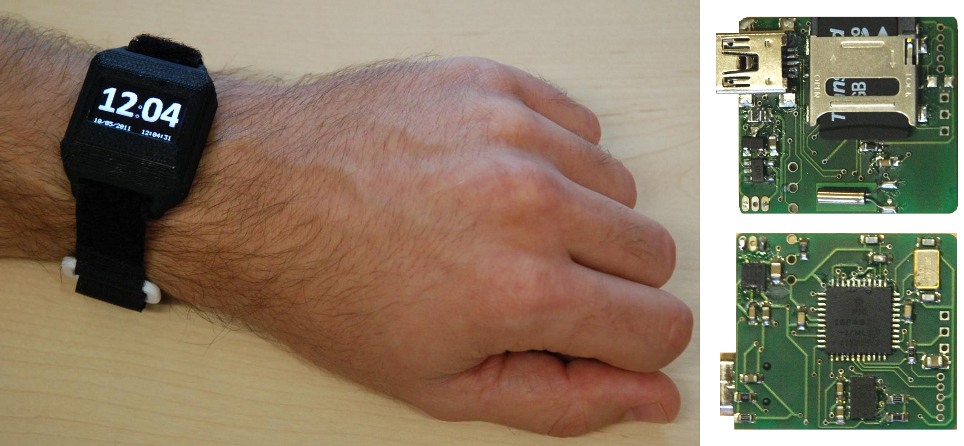
\includegraphics[width=\textwidth]{Images/hardware_sensor_2.jpg}
	\caption{The inertial data logger featuring a low-power microcontroller, a 3 axis accelerometer, a microSD flash card for storing the sensor data and a USB connector for accessing the stored data (on the right) is being powered by a small lithium polymer battery and is packaged into a plastic case to be worn at the wrist (a version with a OLED display on the left).}
	\label{fig:sensornode}
\end{figure}

The 3D accelerometer sensor is being sampled at $100Hz$, resulting in 10ms equidistant measurements. For efficiency reasons, the sensor data is run-length encoded before being stored locally to the microSD card. The HedgeHog can be extended with further sensors tailoring different application scenarios. For our scenario, we have added a capacitive proximity sensor, which is described in detail in the next section.

\subsection{Capacitive Proximity Sensor}

The capacitive proximity sensor performs measurements in loading mode. Two electrodes are integrated into the wristband, one sensing electrode and one shielding electrode that aims to eliminate the influence of the arm that is a very proximate grounded object to the sensing electrode. The sensor draws a supply current of 1 mA at 3.3 V when active. This low power consumption qualifies the sensor for wearable proximity sensing applications. 

\begin{figure}
	\centering
		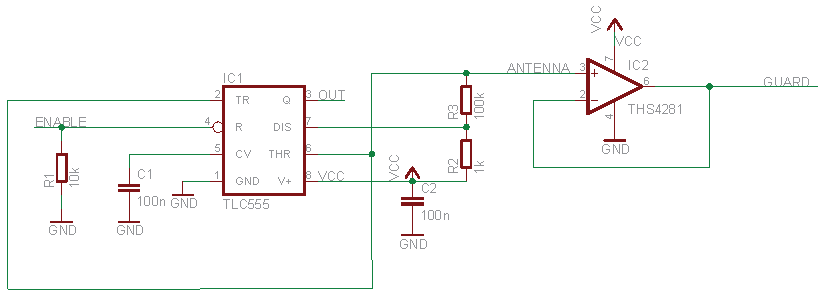
\includegraphics[width=1.00\textwidth]{Images/schematic.pdf}
	\caption{The sensing circuit is based on a timer with an operational amplifier that acts as a voltage follower. The wire that is labeled with ``antenna'' leads to the sensing electrode, whereas the wire labeled with ``guard'' leads to the shield electrode.}
	\label{fig:schematic}
\end{figure}

The sensing circuit schematic is shown in Figure \ref{fig:schematic}. It is based on a timer that controls the charging and discharging cycles of the virtual capacitor that is built by the sensing electrode and the surrounding environment. The timer toggles from charge to discharge at the time when a threshold voltage at the capacitor is reached. This results in an astable operation with succeeding charge/discharge cycles. When the capacitance of the virtual capacitor increases, the charging time will also increase and vice-versa. Therefore, the capacitance is inversely proportional to the number of charging cycles in a given time span. In order to guard the sensor from measuring the capacitance to underlying objects, a shield electrode is placed directly underneath the measuring electrode. The shield is driven with the same potential as the sensing electrode, such that the the capacitance between the two electrodes is negligible. Using this shielding method the measured capacitance will only be slightly affected by the grounded underlying arm.

\begin{figure}
	\centering
		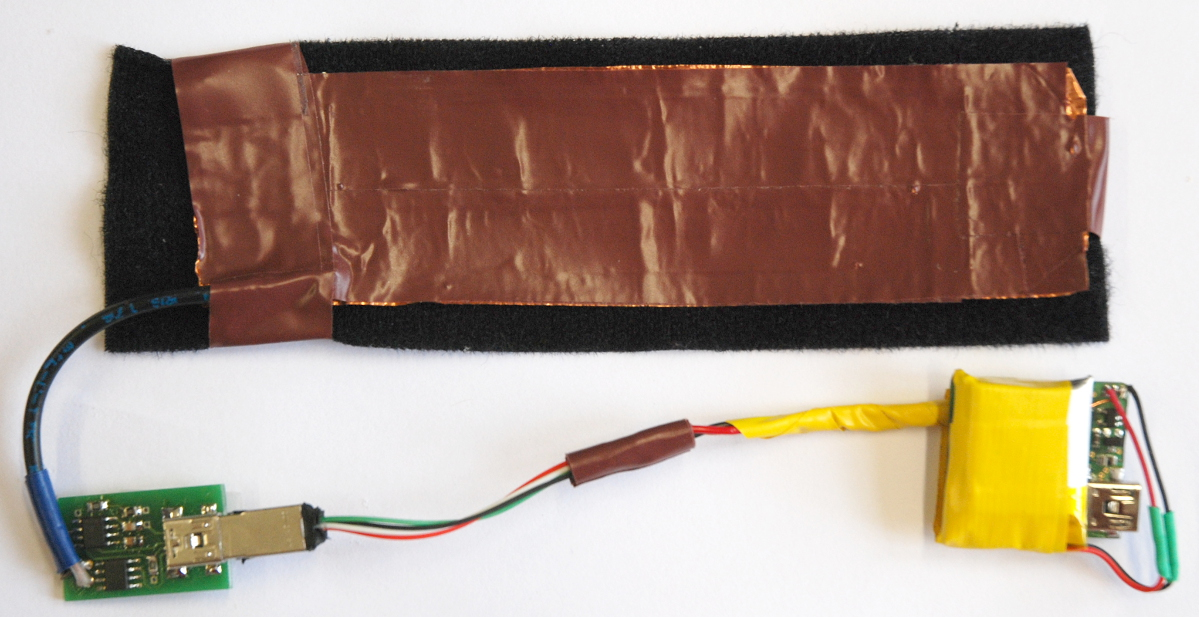
\includegraphics[width=1.00\textwidth]{Images/capacitive_sensor_wristband_2.jpg}
	\caption{The hardware prototype at a glance: HedgeHog activity logger at the lower right, the capacitive sensor unit at the lower left, and the wristband with the sensing and the shield electrodes on-top each other covered with adhesive tape for isolation purposes.}
	\label{fig:cap_sensor}
\end{figure}

Figure \ref{fig:cap_sensor} shows the the wrist-worn prototype used in the evaluation experiments, with the HedgeHog as the main data logger, the capacitive sensor circuit and the wristband holding the sensing and shielding electrodes.

\begin{figure}
	\centering
 		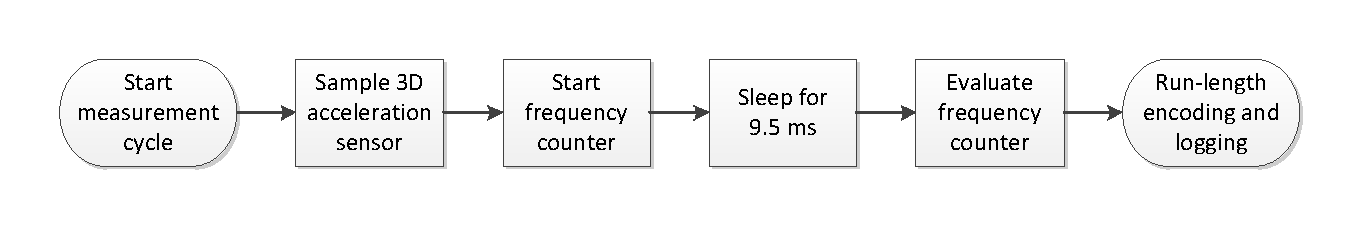
\includegraphics[trim=1cm 1cm 1cm 1cm,clip,width=\textwidth]{Images/pseudocode.pdf}
	\caption{Measurement procedure carried out by the HedgeHog sensor: using the microcontroller's Timer0 module in counting mode, the oscillating signal generated by the capacitive sensor circuit can be measured by counting the frequency pulses over a predefined gate time (approximately 9.5ms).}
	\label{fig:pseudocode}
\end{figure}

Figure \ref{fig:pseudocode} illustrates the operations required for a measurement cycle. The proximity sensor board generates a clock signal with varying frequency depending on the charge and discharge cycles. The HedgeHog measures the resulting capacitance by counting the signal's edges over a gate time of approximately 9.5ms. During that counting phase, the HedgeHog is sent to sleep in order to reduce power consumption. In the following, the HedgeHog applies run-length encoding on the measured data to reduce overhead and periodically logs the data to the integrated SD card.

\section{Experiment}
\label{sect:experiment}

This section presents the experimental setup including the activities and the participants, as well as the findings that were obtained during the evaluation.

\subsection{Setup and Scenario}

The experiment setup aims to depict a typical scenario in daily life. Especially in the field of Ambient Assisted Living (AAL), it is desired to monitor activities like drinking, preparing lunch and sleeping. A fine-grained monitoring of such activities may help elderly or people suffering from mental diseases to maintain a healthy day/night rhythm and take action if irregularities occur. Figure blubb shows the modified HedgeHog activity logger that has been extended with a capacitive proximity sensor. The wristband has two electrodes, a sensing electrode underneath a slightly bigger shield electrode. 

The recorded test set contains the following activities: opening door, sitting on a couch, lying on a couch, grasping into a locker, sitting at the table, preparing a bread with marmalade, eating the bread, drinking water and sleeping. Some of those activities are very hard to recognize without any further contextual information, when the data is limited to a single modality like a 3D accelerometer. For example, sitting at the table and sitting on a couch are very similar activities. We aim to show that the data basis can be significantly improved by the additional input modality. 

In order to evaluate if capacitive proximity sensors in wrist-bands can enhance the performance of activity recognition, we have conducted an evaluation with 7 test persons. All test persons received a basic plot with the activities they were supposed to perform. They were not given any instructions about the way they are supposed to perform the activities. After manual labeling, we used this test-set as ground truth and performed a 4-fold cross-validation on an support-vector machine (SVM) classifier on each user, once with and once without including the data of the capacitive proximity sensor into the feature set. We used an SVM classifier because of its high relevance in activity recognition and its fast performance. 

The classifier was trained with various features that were extracted from windows with the length of 1 second. It turned out that greater window sizes do not provide better results. In order to suppress noise contained in the capacitive proximity sensing data, we applied a moving average filter with a kernel size of 10. The final feature set contained the arithmetic mean, min, max, median and standard variance of both accelerometer and proximity data. These simple feature types represent standard features applied in activity recognition. 

\subsection{Evaluation Results}
\label{sect:evaluation}

In the following, the performed activities will be analyzed in detail, stating out the influence of the capacitive proximity sensor on the classification result. In general, the usage of data provided by the new modality showed improvements in recognition rates by 2.4 - 14.4 \%.

\begin{figure}[htbp]
	\centering
		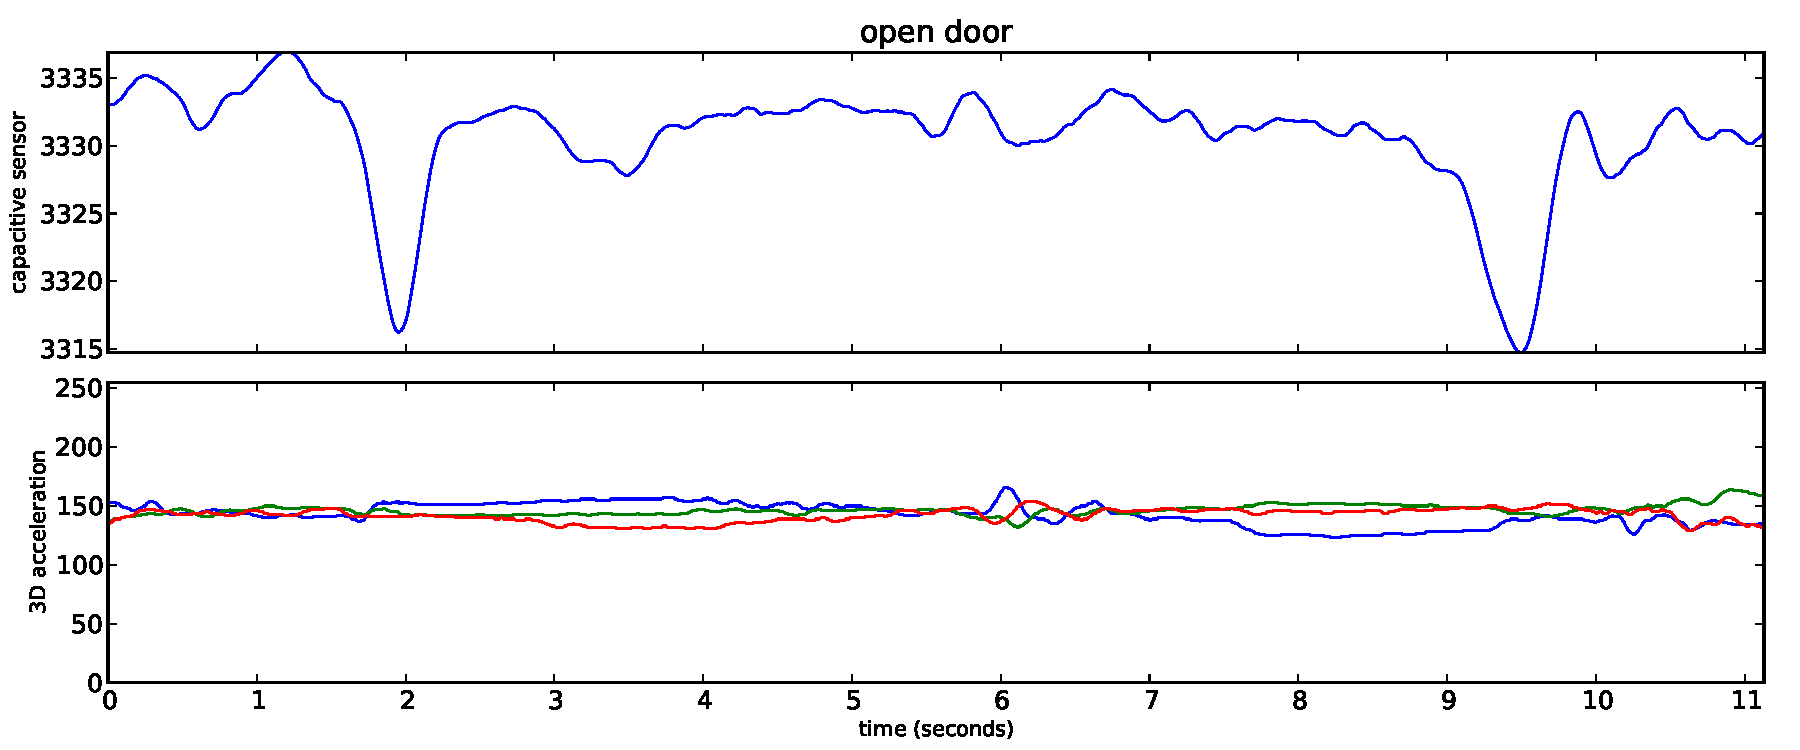
\includegraphics[width=1.00\textwidth]{../Auswertung/images/tobias_1.pdf}
	\caption{While entering the door, the wristband approaches the door knob twice, while opening and closing. Regarding the capacitive proximity sensor, this situation can be observed at the beginning and at the end of the activity.}
	\label{fig:tobias_1}
\end{figure}

The opening door activity has very poor recongition rates without the including the proximity sensor. The average f-measure could be increased from of 34.2 \% to 46.8 \%. A plot of the activity is given in Figure \ref{fig:tobias_1}. The capacitive proximity sensor shows two approaches to the door knob, one for opening the door (2 s) and one for closing the door (9 s). The acceleration sensor captures relevant data in the time in which the person moves into the room and the hand changes from the outer to the inner door knob (5 - 7 s). The recorded data for this activity shows strong correlations between all test persons. The confusion matrices show that the open door activity was often mixed up with the sitting activity because of the horizontal orientation of the hand. Due to the usage of the capacitive sensor, the recall for that class and confusion with the sitting activity improved. 

\begin{figure}[htbp]
	\centering
		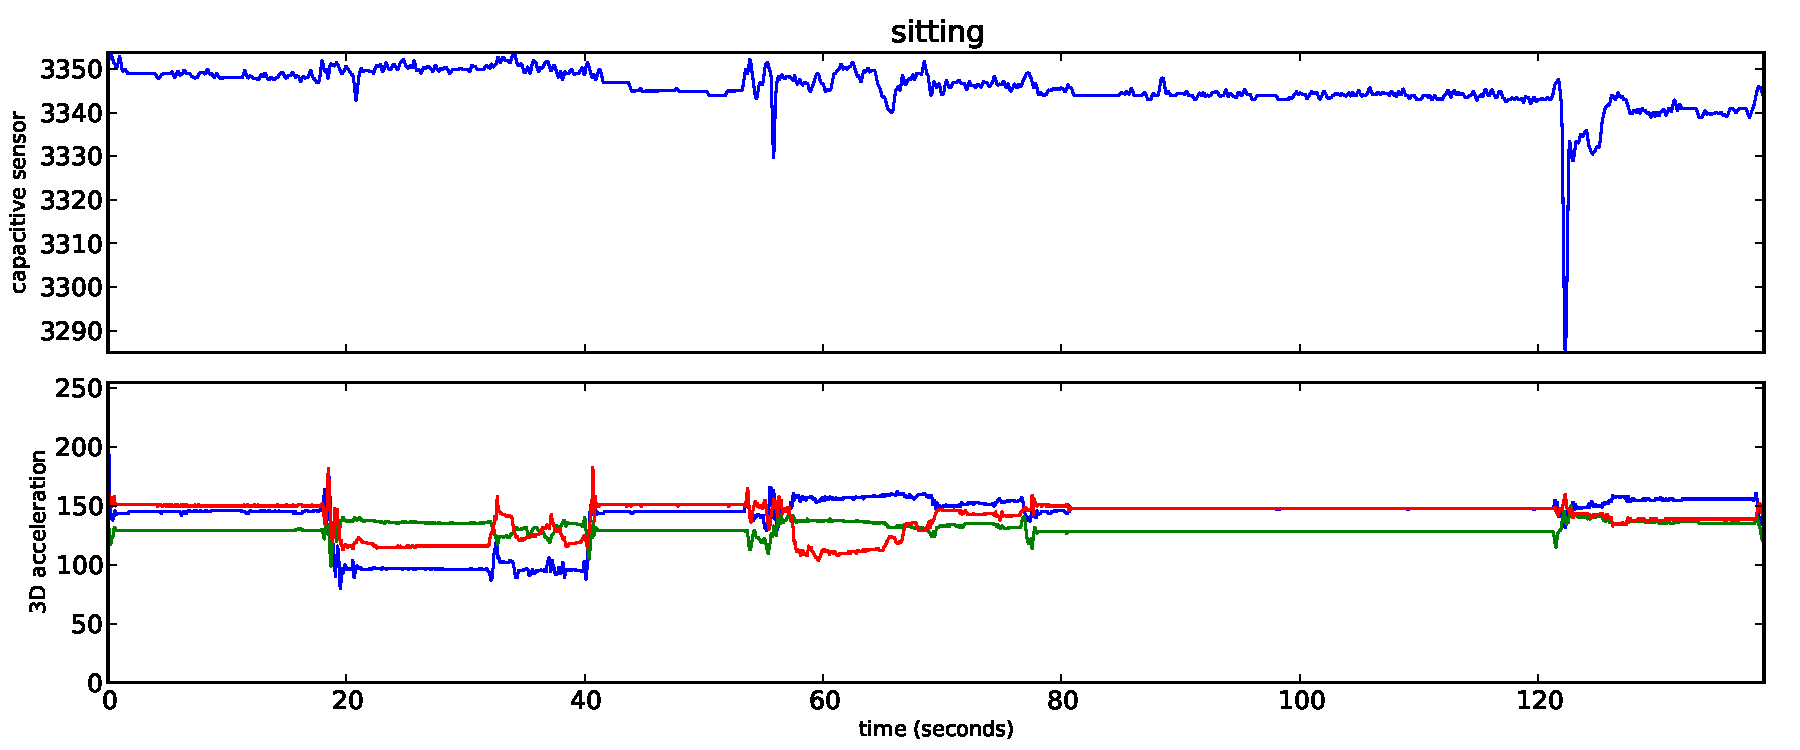
\includegraphics[width=1.00\textwidth]{../Auswertung/images/eugen_2.pdf}
	\caption{Example of a ``sitting'' activity in which user changed his position very frequently. Throughout the whole activity the values of the proximity sensor stay constant due to the close proximity to the couch's fabric.}
	\label{fig:eugen_2}
\end{figure}

After closing the door, the test persons were supposed to sit down on the couch. It turned out that there are great variations of the sitting posture and the corresponding hand positions. Many users tapped with their fingers or hands while sitting, and changed their sitting positions very frequently as shown in Figure \ref{fig:eugen_2}. In this case, it is obvious that the data from the acceleration sensor is very difficult to interprete as there are numerous changes in the axial orientation of the sensor. However, the capacitive proximity sensor is able to indicate when a hand is placed on the surface of the couch. Especially for this test person, the f-measure increased from 27.4 \% to 66.7 \%, while the average f-measure improved from 68.1 \% to 77.6 \%. 

In the following, the test persons were supposed to lay down on the couch. Again, there were great variations in performing this activity between all participants. For example, some of them crossed their hands under their head. For that class, the average f-measure could only be increased by 2.4 \%, from 82.1 to 84.5 \%. Considering some test persons, this class was confused with the make bread activity and could be improved by the proximity sensor. 

The participants were also asked to put food and dishes from a shelf and a locker on a table. The capacitive proximity sensor captured the proximity to the shelf and to the table. The overall f-measure for this activity is rather low, but improved by 6.7 \% from 50.4 \% to 57.1\%. Reasons???

\begin{figure}[htpb]
	\centering
		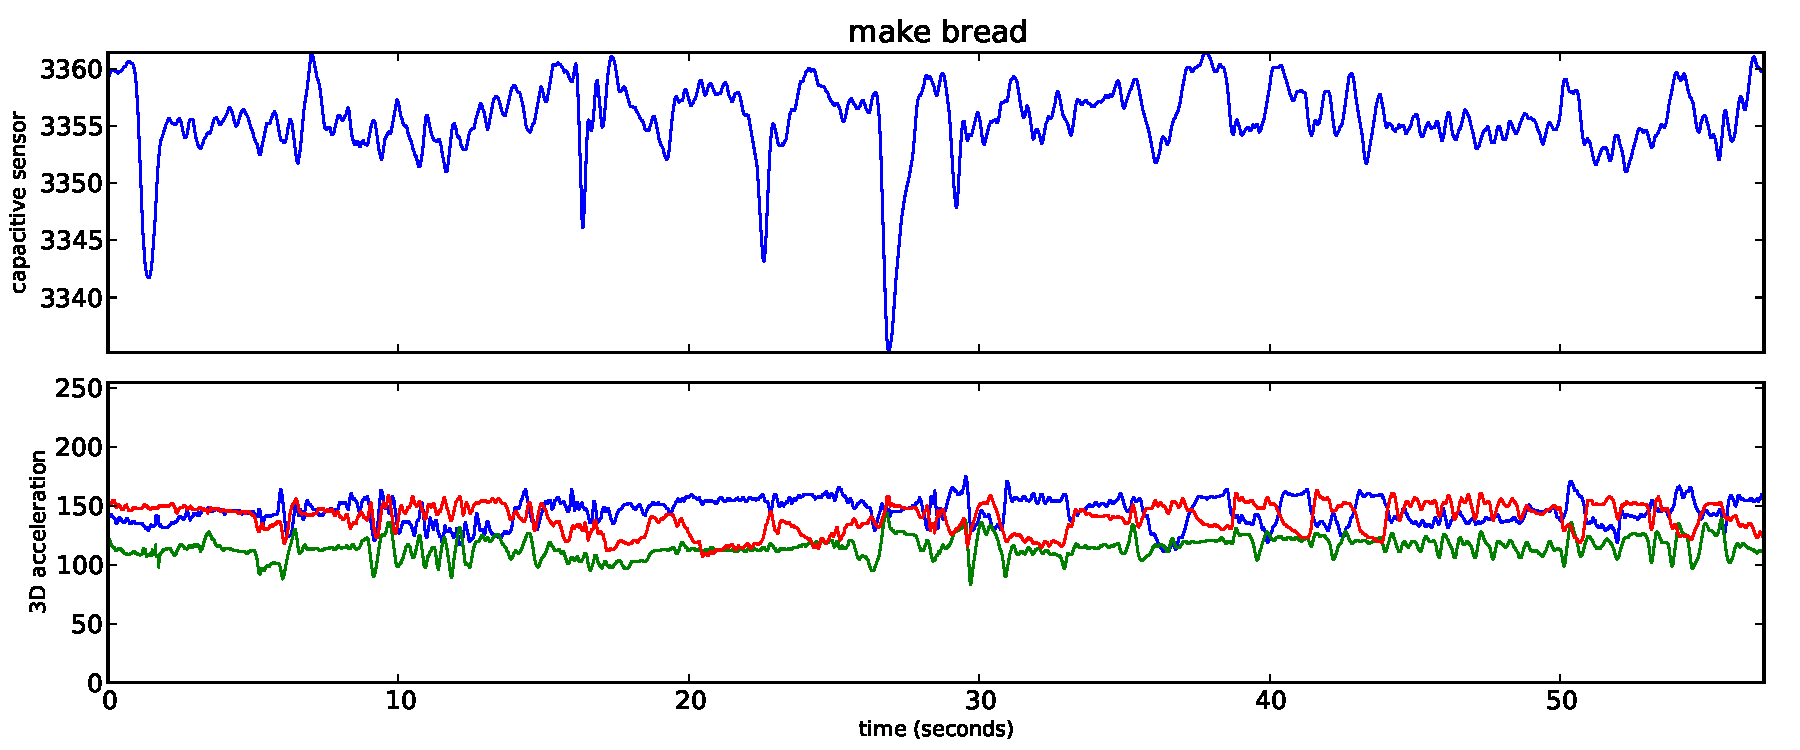
\includegraphics[width=\textwidth]{../Auswertung/images/eugen_5.pdf}
	\caption{An example of the ``preparing bread'' activity, where the participants had to put marmalade on a toast. The proximity sensor indicates the closeness to the table, while the acceleration sensor shows reoccurring movements.}
	\label{fig:eugen_5}
\end{figure}

Figure \ref{fig:eugen_5} shows an example instance of preparing a bread with marmelade. It is notable that the acceleration data does not seem to provide any characteristic patterns, while the proximity sensor indicates a table, plate, or other objects in immediate distance. This activity showed a high improvement in the average f-measure by 10 \%, from 49.0 \% to 59.8 \%, when the data delivered by the capacitive proximity sensor is taken into account. The making bread class was often confused with the sitting class. Using the new input modality, this confusion could be improved.

\begin{figure}[htpb]
	\centering
		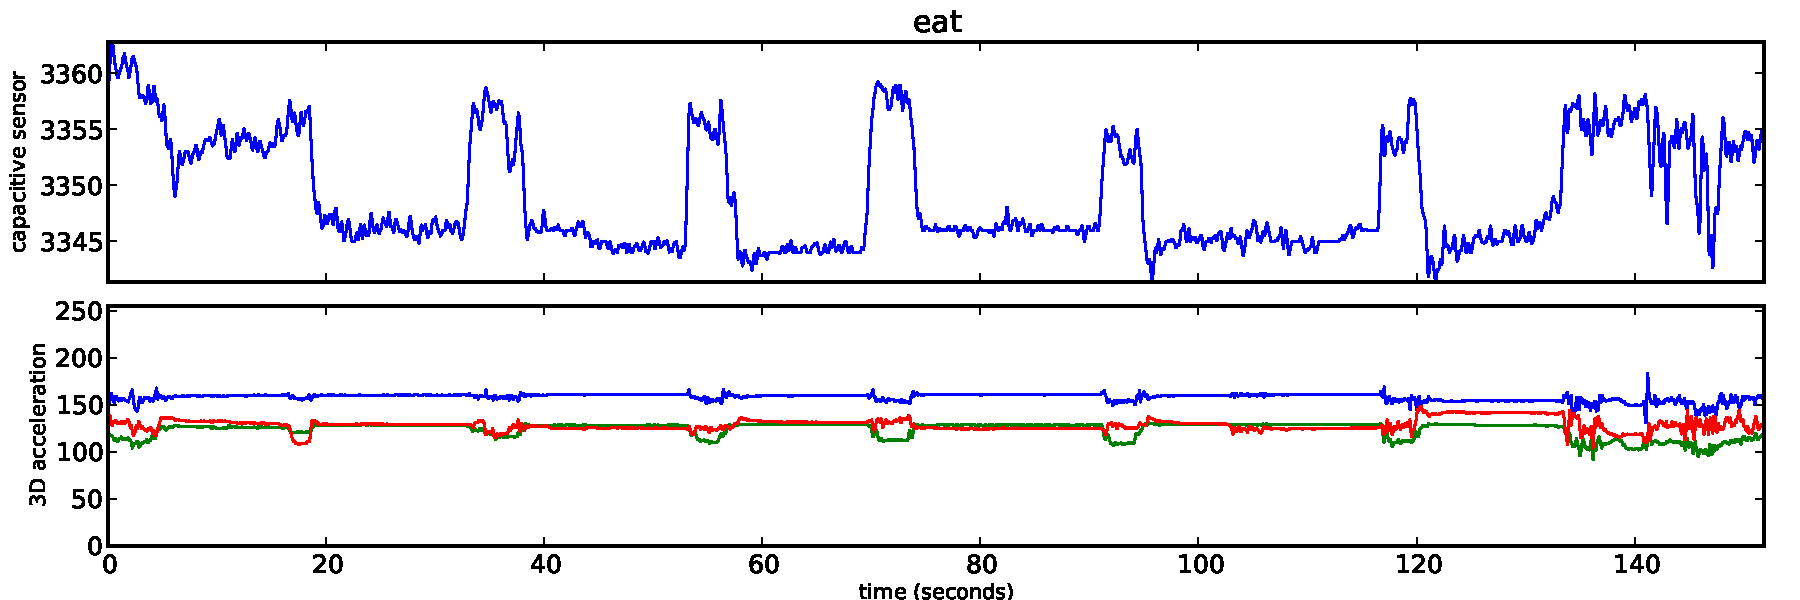
\includegraphics[width=\textwidth]{../Auswertung/images/eugen_6.pdf}
	\caption{An eating person who took 5 bites from the bread. After each bite, the hand is placed on the table.}
	\label{fig:eugen_6}
\end{figure}

Considering the eating activity, the influence of the capacitive proximity sensor is very low. Some of the participants ate their bread leaving their hand close to the mouth, while others moved their hand up and down putting their bread aside on the plate. A good example of an eating activity is shown in Figure \ref{fig:eugen_6} where the participant took a few bites from the bread. The average f-measure for that activity increased slightly from 80.3 \% to 83.8 \%. 

\begin{figure}[htpb]
	\centering
		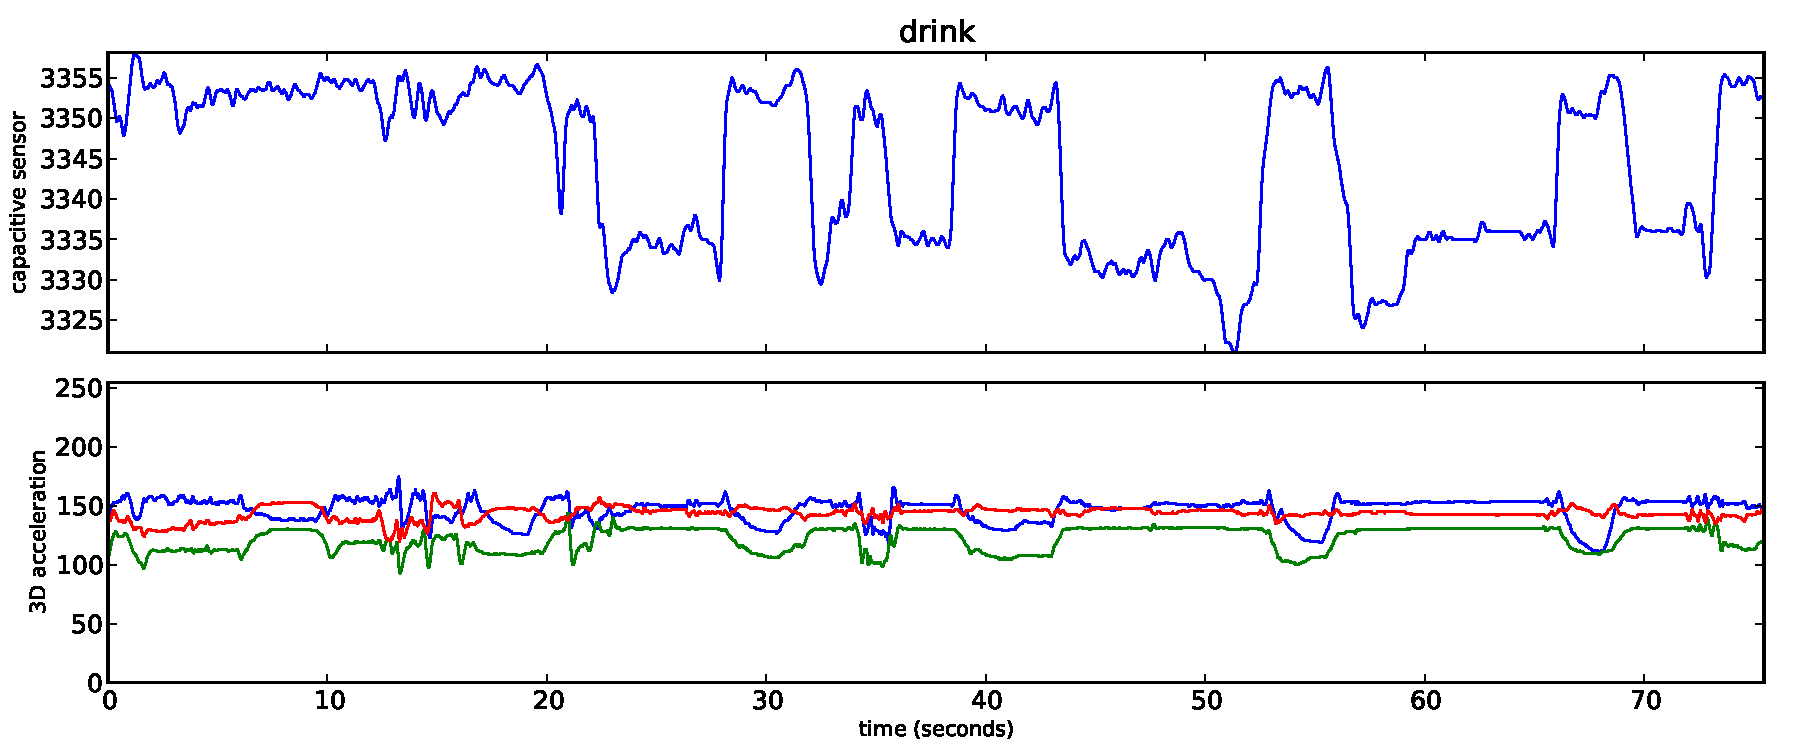
\includegraphics[width=\textwidth]{../Auswertung/images/eugen_7.pdf}
	\caption{An example of the ``drinking'' activity of a test person. The participant first pours some water into the glass and then takes three drams of water. After each dram, he returns his arm to the table which can be observed in the characteristic patterns of the proximity sensor.}
	\label{fig:eugen_7}
\end{figure}

The activity drinking water is depicted in Figure \ref{fig:eugen_7}. The participant took a few nips from the glass, while leaving the hands lying on the table in between. These motions can be easily detected in the acceleration as well as proximity data. The accelerometer data shows that there periodic up- and down-movements while the capacitive proximity sensor delivers data that is associated to the proximity of the table.

\begin{figure}[htbp]
	\centering
		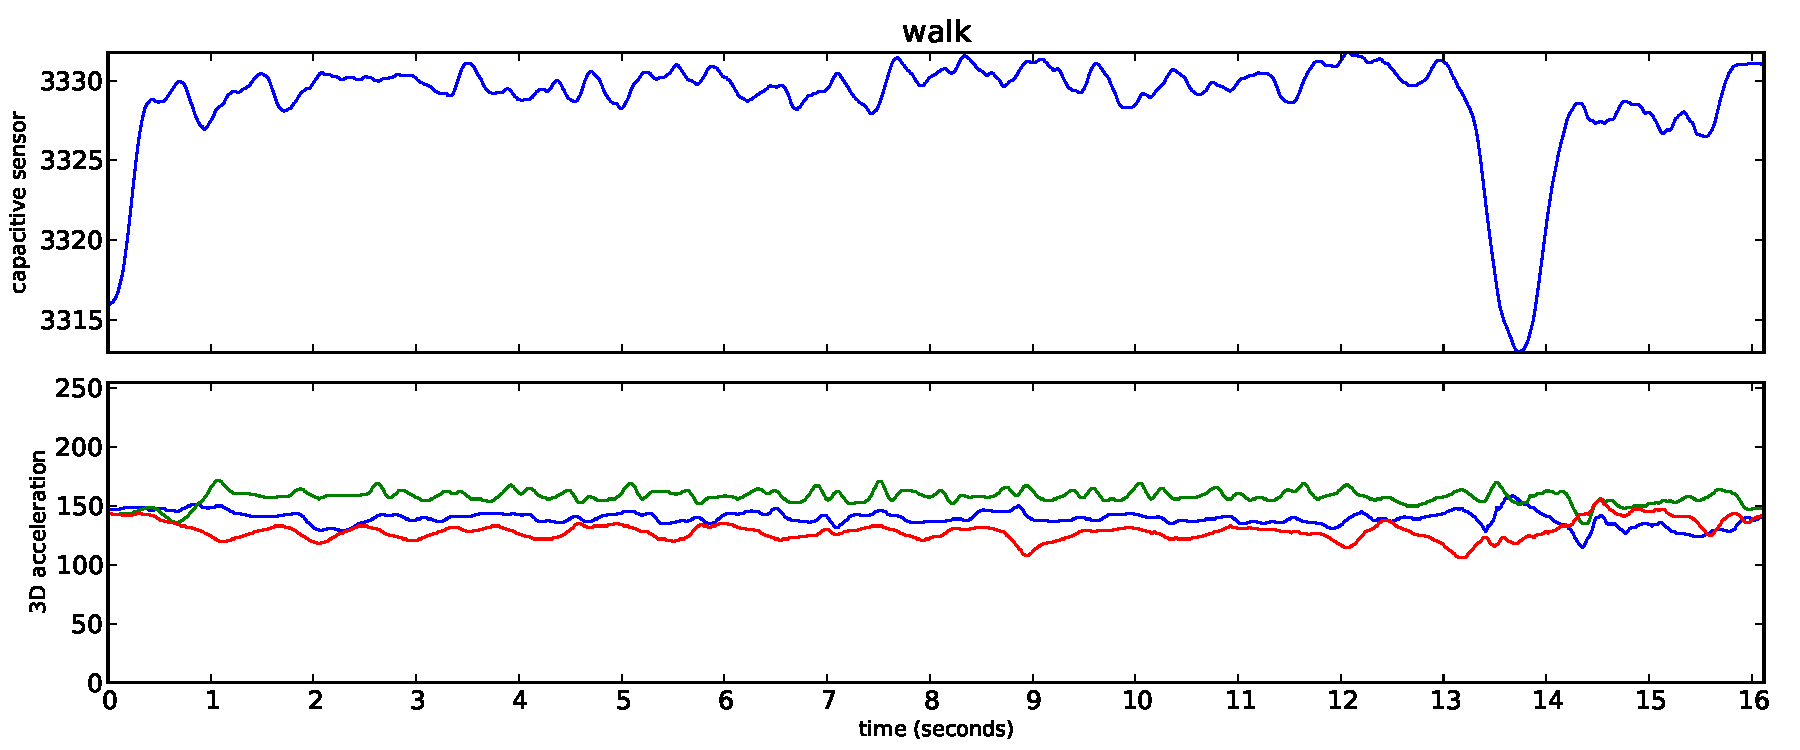
\includegraphics[width=1.00\textwidth]{../Auswertung/images/marko_8.pdf}
	\caption{An examplary instance of the class ``walking''. The acceleration sensor and the proximity sensor show periodic reoccuring patterns that are related to the pendulum-like arm movement and the proximity to the person's body during those movements.}
	\label{fig:marko_8}
\end{figure}

Regarding the walking activity one can identify periodic changes in the acceleration as well as in the measured capacitance, illustrated in Figure \ref{fig:marko_8}. While walking, the capacitance between the wristband and the leg increases when the wristband is located close to the body and decrease when the wristband moves away. There were problems in distinguishing this activity from get things that could be bettered by using the new input modality. 

\begin{figure}[htbp]
	\centering
		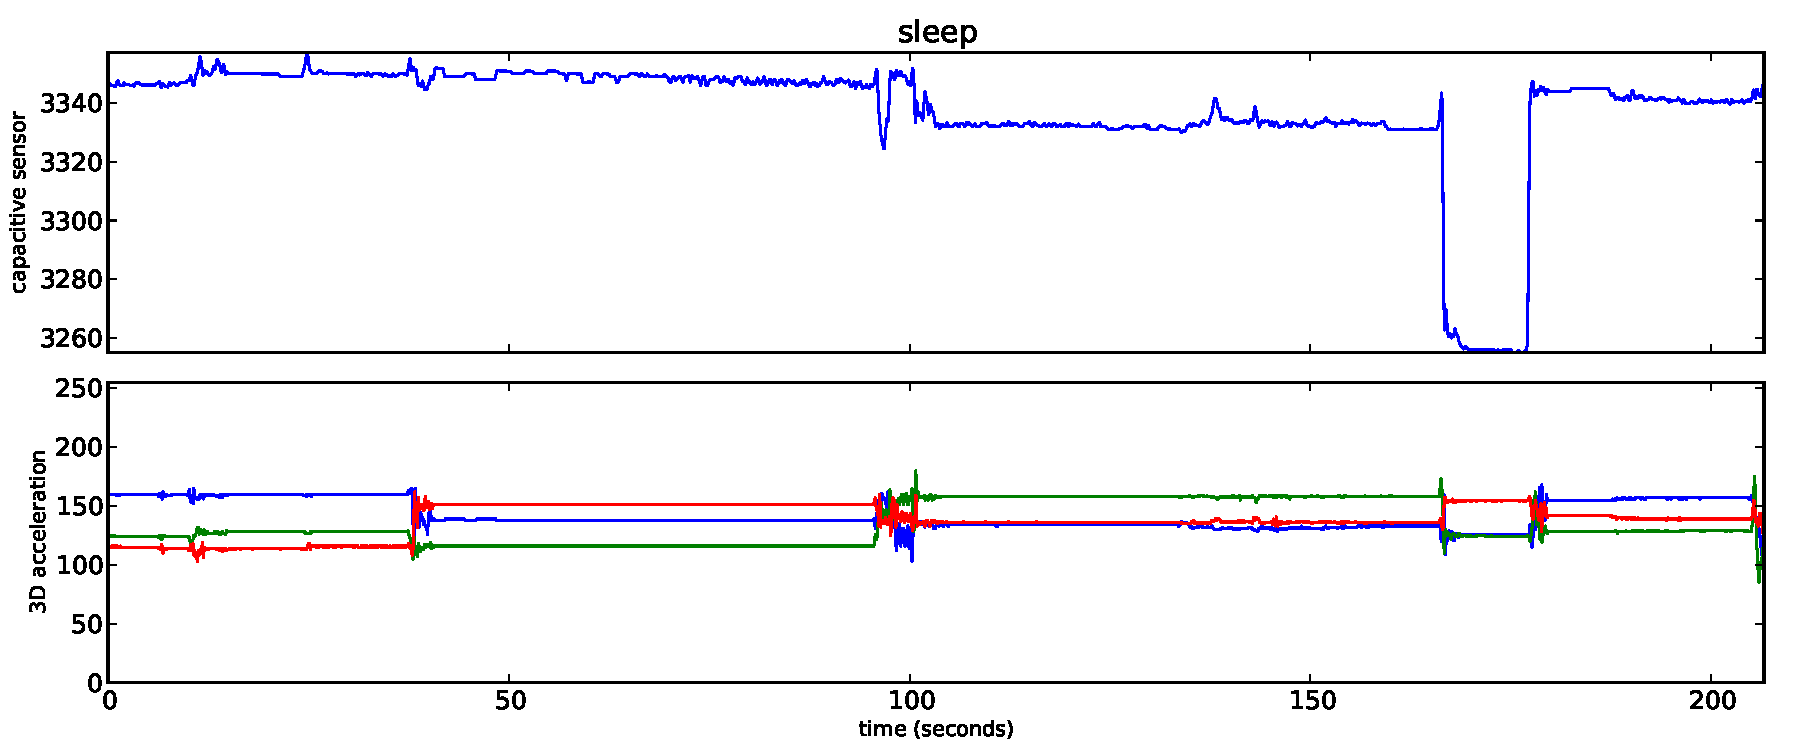
\includegraphics[width=1.00\textwidth]{../Auswertung/images/eugen_9.pdf}
	\caption{During the sleeping activity the data from both sensors remains constant. One draw conclusions about the coverage of the arm with either couchons, blankets or the proximity to the mattress.}
	\label{fig:eugen_9}
\end{figure}

The sleeping activity was captured with an average f-measure of 83.4 \% that increased to 88.4 \% when using the capacitive proximity sensor. In this situation the capacitive proximity sensor is able to capture the surrounding couchons and blankets. The accelerometer data and the proximity data is very constant during that activity. 

\begin{table}[htbp]
	\centering	\begin{tabular}{p{0.48cm}p{0.48cm}p{0.48cm}p{0.48cm}p{0.48cm}p{0.48cm}p{0.48cm}p{0.48cm}p{0.48cm}|p{0.48cm}p{0.48cm}p{0.48cm}p{0.48cm}p{0.48cm}p{0.48cm}p{0.48cm}p{0.48cm}p{0.48cm}|p{2.2cm}}
a & b & c & d & e & f & g & h & i & a & b & c & d & e & f & g & h & i & $\leftarrow$ classified as\\
\hline
10 & 3 & 0 & 2 & 0 & 0 & 0 & 0 & 0 		& 9 & 5 & 0 & 0 & 1 & 0 & 0 & 0 & 0 & a = open door\\
\hline
2 & 259 & 4 & 2 & 4 & 2 & 4 & 0 & 0 	& 1 & 248 & 5 & 6 & 4 & 2 & 5 & 0 & 0 & b = sit\\
\hline
0 & 5 & 213 & 2 & 2 & 1 & 8 & 0 & 4 	& 0 & 3 & 212 & 3 & 2 & 1 & 6 & 0 & 8 & c = lying\\
\hline
3 & 5 & 2 & 52 & 9 & 3 & 1 & 1 & 1 		& 0 & 8 & 2 & 44 & 7 & 8 & 1 & 1 & 3 & d = get things\\
\hline
1 & 9 & 3 & 13 & 46 & 6 & 3 & 0 & 0 	& 1 & 7 & 1 & 11 & 37 & 9 & 2 & 0 & 10 & e = make bread\\
\hline
0 & 5 & 1 & 1 & 5 & 62 & 5 & 0 & 1 		& 0 & 3 & 2 & 3 & 8 & 58 & 5 & 0 & 1 & f = eat\\
\hline
0 & 8 & 4 & 2 & 1 & 5 & 68 & 0 & 0 		& 0 & 8 & 3 & 0 & 6 & 4 & 67 & 0 & 1 & g = drink\\
\hline
1 & 0 & 0 & 1 & 0 & 0 & 0 & 12 & 0 		& 1 & 0 & 0 & 1 & 0 & 0 & 0 & 13 & 0 & h = walk\\
\hline
1 & 0 & 0 & 7 & 0 & 0 & 0 & 0 & 325 	& 0 & 1 & 2 & 10 & 6 & 1 & 1 & 0 & 312 & i = sleep\\
		\end{tabular}
	\caption{Comparison of two Confusion matrices for an exemplary user. The left part includes the capacitive proximity sensor, the right part represents classification results without the sensor.}
	\label{tab:ConfusionMatrixForAnExemplaryUser}
\end{table}

Table \ref{tab:confmatrix} 

\section{Conclusion and Outlook}
\label{sect:conclusions}

We have shown that current wearable inertial sensing devices for activity recognition can be significantly enhanced by integrating a capacitive proximity sensor into the wristband. Regarding the classification accuracy, we obtained an overall increase in correctly classified instances of TODO percent. Some classes, for instance ``preparing bread'' and ``drinking'', could benefit very much from proximity-related sensor data. For such classes the classification performance could be boosted by up to TODO percent. 

The classification results could be improved by the usage of more than one sensing electrode in the wristband. For example the wristband could integrate four electrodes that are placed on each side of the arm. However, this will lead to smaller electrode surfaces that lead to a decrease of sensing distance. We think that these considerations are an important subject of future work. The sensor's power consumption can be decreased by shorter measurement windows and the choice of more energy efficient hardware components. Measuring pulse width lengths instead of counting the rising edges of the sensor's signal may reduce the required time needed for a measurement.

Capacitive proximity sensors represent a suitable new input modality for future activity recognition systems. The low power consumption as well as the invisible integration of a sensor into the wristband meets an essential requirement of wearable applications. Especially in AAL environments, these systems can help monitoring the course of chronic diseases by recognizing activities of daily life. This may improve the quality of life of persons affected and their caregivers. 

\section*{Acknowledgments}

We would like to thank our evaluation participants from TU Darmstadt and Fraunhofer IGD.

% \newpage

\bibliographystyle{splncs03}
\bibliography{references}

\end{document}
